% journal_ui_ana/indonesia/src/20_pengembangan_hipotesis.tex
% Atau bisa dinamai 20_tinjauan_pustaka.tex jika lebih sesuai
\section{Tinjauan Pustaka dan Landasan Teori} % Judul disesuaikan agar lebih umum untuk jurnal

Rekayasa balik (\f{reverse engineering}) merupakan proses fundamental dalam analisis perangkat lunak yang bertujuan untuk memahami mekanisme internal suatu sistem tanpa akses ke kode sumber aslinya \cite{Has18, gee24}. Proses ini menjadi ancaman signifikan terhadap keamanan perangkat lunak karena dapat dimanfaatkan untuk mengungkap algoritma propietari, mengidentifikasi kerentanan keamanan, membajak lisensi, hingga menyisipkan kode berbahaya \cite{Wak24}. Kelemahan ini mendorong pengembangan berbagai teknik proteksi, di antaranya adalah pengaburan kode (\f{code obfuscation}).

\subsection{Teknik Pengaburan Kode (\f{Code Obfuscation})}
Pengaburan kode bertujuan untuk mentransformasi kode program ke dalam bentuk yang secara fungsional ekivalen namun secara signifikan lebih sulit untuk dipahami dan dianalisis oleh manusia \cite{Jin24}. Tujuannya bukan untuk membuat rekayasa balik mustahil, melainkan untuk meningkatkan kompleksitas dan biaya yang dibutuhkan sehingga menjadi tidak praktis bagi penyerang. Teknik pengaburan dapat diklasifikasikan berdasarkan level abstraksi di mana ia diterapkan:

\subsubsection{Pengaburan Kode Sumber (\f{Source Code Obfuscation})}
Modifikasi dilakukan pada kode sumber yang dapat dibaca manusia.
\begin{itemize}
    \item \bo{Pengaburan Tata Letak (\f{Layout Obfuscation}):} Mengubah tampilan kode, seperti mengacak nama variabel dan fungsi \cite{Cha04}, serta menghapus spasi putih dan komentar \cite{Bal11}. Memberikan tingkat keamanan minimal terhadap analisis otomatis.
    \item \bo{Pengaburan Data (\f{Data Obfuscation}):} Menyembunyikan representasi data, misalnya melalui enkoding \f{string} \cite{Ert05, Fuk08, Kov13}, substitusi instruksi \cite{LeD12, Dar10}, atau penggunaan ekspresi aritmetika-boolean campuran (\f{mixed boolean-arithmetic}) \cite{Liu21, Sch22, Zho07} untuk menyamarkan logika manipulasi data.
    \item \bo{Pengaburan Alur Kontrol (\f{Control Flow Obfuscation}):} Memodifikasi logika alur eksekusi program. Contohnya termasuk penyisipan alur kontrol palsu (\f{bogus control flow}) \cite{LiY211}, penggunaan predikat buram (\f{opaque predicates}) \cite{XuD16}, dan perataan alur kontrol (\f{control flow flattening}) yang mengubah struktur kode menjadi pernyataan \code{switch} besar dan kompleks \cite{Lás09}.
\end{itemize}

\subsubsection{Pengaburan \f{Bytecode} (\f{Bytecode Obfuscation})}
Teknik ini menargetkan kode perantara seperti Java \f{bytecode}, .NET CIL, atau LLVM IR. Metode yang digunakan meliputi penggantian nama pengenal, pengaburan alur kontrol, enkripsi \f{string}, dan penyisipan kode semu (\f{dummy code}) \cite{Pie18, Yak20}. Efektif untuk mempersulit dekompilasi kembali ke kode sumber tingkat tinggi.

\subsubsection{Pengaburan Kode Biner (\f{Binary Code Obfuscation})}
Beroperasi langsung pada kode mesin yang dapat dieksekusi.
\begin{itemize}
    \item \bo{Pengepakan/Enkripsi Kode (\f{Code Packing Encryption}):} Mengompresi atau mengenkripsi kode asli, memerlukan \f{stub} runtime untuk membongkar/mendekripsi kode sebelum eksekusi \cite{Rou13}. Utama menghambat analisis statis, namun kode asli akan terungkap di memori saat eksekusi.
    \item \bo{Manipulasi Alur Kontrol:} Menggunakan lompatan/panggilan tidak langsung, memodifikasi instruksi \code{call}/\code{ret}, atau memecah kode menjadi blok-blok kecil dengan lompatan untuk mengganggu analisis dan \f{disassembly} linier \cite{Rou13}.
    \item \bo{Pengaburan Konstanta:} Menyembunyikan nilai-nilai konstan melalui operasi aritmetika atau logika \cite{Rou13}.
    \item \bo{Virtualisasi Kode (\f{Code Virtualization}):} Dianggap sebagai salah satu teknik pengaburan biner terkuat, yang akan dibahas lebih lanjut.
\end{itemize}

\subsection{Virtualisasi Kode (\f{Code Virtualization})}
Virtualisasi kode, atau pengaburan berbasis Mesin Virtual (VM), adalah teknik canggih di mana segmen kode mesin asli diterjemahkan menjadi format \f{bytecode} khusus. \f{Bytecode} ini kemudian dieksekusi oleh sebuah VM yang dirancang khusus dan disematkan langsung ke dalam aplikasi \cite{Ore06, Zho24}. Seperti yang diilustrasikan pada Gambar \ref{F:jurnal_ui_ana_virtualization_process} dari penelitian Oreans \cite{Ore06}, proses ini mengubah kode asli menjadi serangkaian instruksi virtual.
% Catatan: Anda perlu memastikan Gambar \ref{F:virtualization_process} ada di direktori assets dan path-nya benar
% atau gambar tersebut sudah didefinisikan sebelumnya jika Anda menggunakan referensi silang dari skripsi.
% Jika tidak, Anda bisa menyertakan gambar tersebut di direktori aset jurnal ini.
% Contoh: \includegraphics[width=0.8\textwidth]{../assets/pics/code_virtualization_process.png}

\begin{figure}[H]
	\centering
	\includegraphics[width=0.7\textwidth]{\Assets/code_virtualization_process.png} % Diasumsikan Assets didefinisikan atau path disesuaikan
	\caption{Proses Virtualisasi Kode \cite{Ore06}}
	\label{fig:jurnal_ui_ana_virtualization_process} % Label unik untuk jurnal
\end{figure}

Lapisan abstraksi yang diperkenalkan oleh VM ini menciptakan penghalang signifikan bagi perekayasa balik. Alat analisis standar tidak dapat secara langsung menginterpretasikan ISA \f{bytecode} yang unik tersebut \cite{Salwan2018SymbolicDeobfuscation}. Perekayasa balik harus terlebih dahulu memahami arsitektur VM, implementasi \f{handler} instruksi virtual, dan pemetaan \f{bytecode}, sebuah tugas yang kompleks dan memakan waktu \cite{Don20, Hac24}.

Beberapa aspek kunci dari pengaburan berbasis VM meliputi:
\begin{itemize}
    \item \bo{ISA Kustom:} Setiap aplikasi yang dilindungi berpotensi memiliki set instruksi virtual yang unik atau termutasi, mempersulit deteksi berbasis \f{signature} atau penggunaan ulang hasil analisis. Oreans \cite{Ore06} menyoroti kemungkinan untuk menghasilkan VM yang beragam untuk salinan aplikasi yang berbeda yang dilindungi.
    \item \bo{Arsitektur VM:} Komponen VM tipikal mencakup unit \f{fetch, decode, dispatch}, dan \f{handler}, meniru operasi CPU namun diimplementasikan dalam perangkat lunak \cite{Salwan2018SymbolicDeobfuscation, Hac24}. Kompleksitas dan detail implementasi dari \f{handler-handler} ini secara langsung memengaruhi keamanan dan performa. Alur eksekusi virtualisasi kode dapat dilihat pada Gambar \ref{fig:jurnal_ui_ana_execution_virtualization} (diadaptasi dari \cite{Don20}).

    \begin{figure}[H]
        \centering
        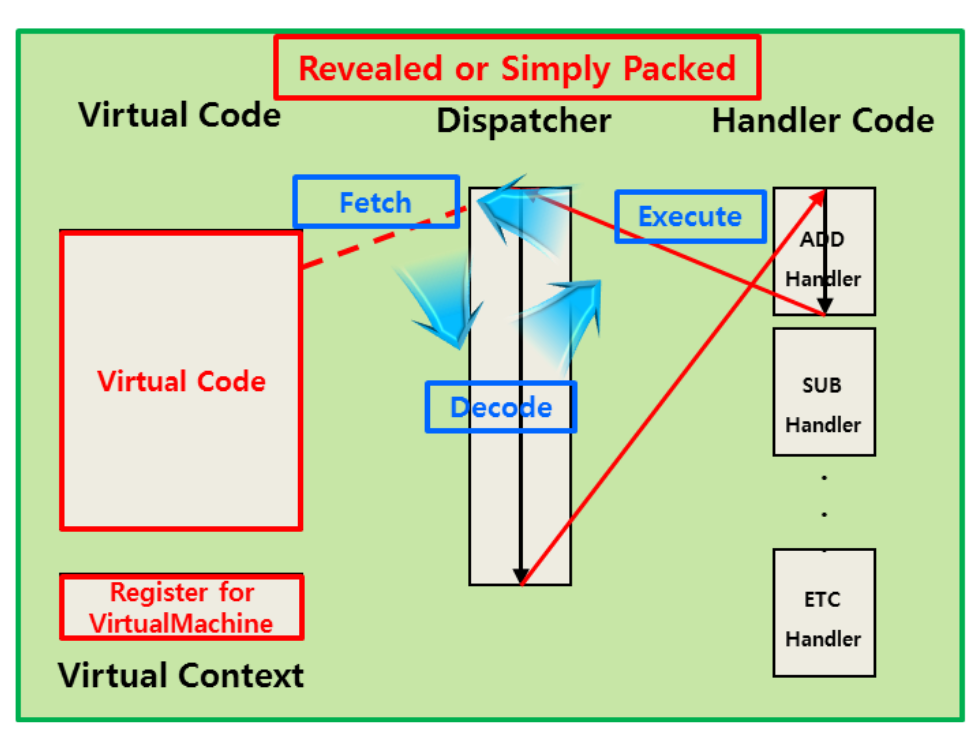
\includegraphics[width=0.6\textwidth]{\Assets/virtualization_execution.png}
        \caption{Alur Eksekusi Virtualisasi Kode (diadaptasi dari \cite{Don20})}
        \label{fig:jurnal_ui_ana_execution_virtualization}
    \end{figure}

    \item \bo{\textit{Trade-off} Keamanan vs. Performa:} Lapisan interpretasi yang diperkenalkan oleh VM secara inheren menambah \f{overhead} performa dibandingkan eksekusi asli. Tingkat pengaburan dalam \f{handler} VM dan kompleksitas instruksi virtual memengaruhi \textit{trade-off} ini.
\end{itemize}

Beberapa alat komersial seperti VMProtect \cite{VMP24} dan Themida \cite{Ore24} (yang juga mencakup fitur virtualisasi di luar pengepakan dasar) menggunakan virtualisasi kode. Penelitian akademis juga telah mengeksplorasi teknik seperti deobfuscation simbolik untuk menganalisis kode tervirtualisasi \cite{Salwan2018SymbolicDeobfuscation} dan metode untuk meningkatkan ketahanan virtualisasi, seperti \f{virtual code folding} \cite{Don20}.

\subsection{Teknik dan Tantangan \f{Disassembly}}
Memahami efektivitas pengaburan biner, khususnya virtualisasi kode, memerlukan tinjauan singkat tentang teknik \f{disassembly}. \f{Disassembler} menerjemahkan kode mesin menjadi bahasa \f{assembly} yang dapat dibaca manusia, membentuk landasan rekayasa balik \cite{Sikorski2012}.

\subsubsection{\f{Disassembler} Statis}
\f{Disassembler} statis, seperti Ghidra \cite{Nat19} dan IDA Pro \cite{Hex91}, menganalisis berkas \f{executable} tanpa menjalankannya. Mereka menggunakan teknik seperti sapuan linier (\f{linear sweep}) atau penelusuran rekursif (\f{recursive traversal}) untuk mengidentifikasi urutan instruksi \cite{Eilam2011, Ko2007}. Meskipun komprehensif, analisis statis kesulitan menghadapi kode yang terenkripsi, dikemas, memodifikasi diri sendiri, atau ditransformasi secara signifikan, karena \f{disassembler} dapat salah menginterpretasikan data sebagai kode atau gagal mengikuti alur kontrol yang sebenarnya \cite{Sikorski2012, Blazytko2017}. Yang krusial, ketika dihadapkan dengan \f{bytecode} kustom dari VM, \f{disassembler} statis yang dirancang untuk ISA standar (misalnya, x86-64) tidak dapat menginterpretasikan instruksi non-natif ini dengan benar, yang menyebabkan kegagalan analisis.

\subsubsection{\f{Disassembler} Dinamis}
\f{Disassembly} dinamis, biasanya merupakan fitur dari \f{debugger} seperti x64dbg \cite{Dun14}, terjadi selama eksekusi program. \f{Debugger} me-\f{disassemble} instruksi secara \textit{on-the-fly} saat akan dieksekusi oleh CPU. Pendekatan ini dapat mengatasi beberapa keterbatasan analisis statis, seperti mengungkapkan kode yang dibongkar atau didekripsi di memori \cite{Sikorski2012}. \f{Debugger} juga dapat mengakses informasi simbol \textit{runtime} yang dimuat oleh sistem operasi untuk pustaka sistem, memberikan konteks untuk panggilan API. Namun, meskipun \f{debugger} dapat melangkah melalui instruksi natif dari \textit{interpreter} VM yang tersemat, ia tidak akan secara langsung mengungkapkan logika asli aplikasi sebelum virtualisasi. Sebaliknya, ia menunjukkan operasi internal VM yang mengeksekusi \f{bytecode} kustom, yang masih mengaburkan semantik inti aplikasi dari analis. Keterbatasan inheren dari alat \f{disassembly} standar ini menggarisbawahi tantangan yang ditimbulkan oleh teknik pengaburan canggih seperti virtualisasi kode.

\subsection{VxLang dalam Konteks}
VxLang memposisikan dirinya sebagai kerangka kerja komprehensif yang menawarkan proteksi biner, pengaburan kode (termasuk \f{flattening}), dan virtualisasi kode \cite{VxLang}. Pendekatannya melibatkan transformasi kode x86-64 asli menjadi \f{bytecode} internal yang dieksekusi oleh VM-nya. Studi ini bertujuan untuk memberikan evaluasi empiris terhadap efektivitas komponen virtualisasi VxLang terhadap praktik rekayasa balik standar dan mengukur biaya performa terkait, sehingga menyumbangkan wawasan praktis tentang kegunaannya sebagai mekanisme proteksi perangkat lunak. Berbeda dengan analisis protektor komersial yang sudah mapan, penelitian ini berfokus pada implementasi spesifik dan dampak dari kerangka kerja VxLang.
